\chapter{Visualizing Static Input Graphs}
\label{chap:visualizing-static-input-graphs}

In this chapter we provide a detailed description of our problem statement, formalize it, and discuss our solution in the case of static input graphs.

Our goal is to visualize clusters of a larger graph, such as an opinion network, as an artificial map. In this map, each cluster of the larger graph is represented by a contiguous region whose area is approximately proportional to the cluster's size, and neighboring regions indicate similarities between the respective clusters.

Unlike OpMap and GMap, which have similar goals, clustering the larger graph is not part of the framework we discuss here. Instead, we assume the larger graph is clustered externally before feeding it into our framework. In a first step, we take the already clustered graph as input and build an initial polygonal contact representation of said graph. Obviously, this is only possible under a few conditions that we formalize in a bit. We then tweak the polygonal contact representation, displacing the polygons' corners in such a way that their areas are approximately proportional to the cluster's sizes and they have somewhat organic shapes. To formalize this, we require two short definitions:

\begin{definition}
	A weighted contact representation is \emph{approximately area-proportional} if its regions' areas are approximately proportional to the weights prescribed by the weight function.
\end{definition}

\begin{definition}
	Given a plane graph $G$, a contact representation of $G$ with simple polygons is called a \emph{polygonal dual} of $G$. A polygonal dual respects the combinatorial embedding and outer face of $G$, \ie{} the regions corresponding to vertices that lie on the outer face of $G$ have a boundary with the implicit outer face of the polygonal dual, and the cyclic order of incident faces is as prescribed by the combinatorial embedding of $G$.
\end{definition}

Unless otherwise noted, we assume that polygonal duals respect the combinatorial embedding and outer face of their primal graphs and that two regions share at most one continuous border, \ie{} the points where two regions meet lie on a single polyline. Note that polygonal duals are a generalization of rectilinear duals and that, analogous to rectilinear duals, a polygonal dual can be interpreted as plane graph itself: the polygons' corners translate to vertices in this graph, and their sides translate to edges.

With these definitions in place, we can formalize the structure of our algorithmic pipeline: Our input is a plane 2-connected, internally triangulated, and vertex-weighted graph, the \emph{cluster graph} $G_\text{emb}$. We start with forming an initial weighted polygonal dual of $G_\text{emb}$'s embedding, the \emph{initial map graph} $G_\text{init}$. $G_\text{init}$ inherits its (face) weights from $G_\text{emb}$'s vertices. We then turn $G_\text{init}$ into an approximately area-proportional, polygonal contact representation of $G_\text{emb}$ with other aforementioned region features, the \emph{(approximately area-)proportional map graph} $G_\text{prop}$. This is done by displacing its vertices while preserving the graphs's planarity. We implement this step using a force-directed algorithm.

\begin{figure}[H]
	\centering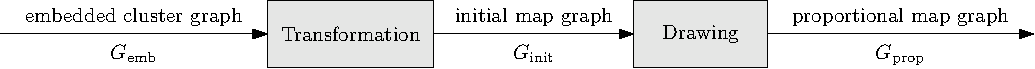
\includegraphics[width=0.9\textwidth]{Resources/Pipeline-Thesis-Static.pdf}
	\caption{Overview of the algorithmic pipeline for static input graphs.}
	\label{fig:static-pipeline-thesis}
\end{figure}

Let's break down the requirements we impose on the cluster graph $G_\text{emb}$ and its embedding:

\begin{itemize}
	\item $G_\text{emb}$ is given as a plane graph. $G_\text{emb}$ must be planar such that there exists a contact representation of $G_\text{emb}$. We require a combinatorial embedding of $G_\text{emb}$ with prescribed outer face such that the \quoted{arrangement} of the clusters or of the regions on the eventual map is predetermined. This becomes important in \cref{chap:visualizing-dynamic-input-graphs} where we start incorporating dynamic updates into the embedded cluster graph and the map graphs.
	\item $G_\text{emb}$ is internally triangulated such that the map graphs $G_\text{init}$ and $G_\text{prop}$ are hole-free. Applying the map metaphor, this translates to there not being any lakes or rivers separating countries on the map. \cref{fig:preliminaries-rectilinear-dual} illustrates how internal faces on 4 or more vertices creates holes in contact representations.
	\item $G_\text{emb}$ is 2-connected such that, in combination with the internal triangulatedness, no vertex appears on outer face multiple times. This is required for how we compute the initial map graph and will be discussed in detail in \cref{sect:transformation-to-dual}.
	\item $G_\text{emb}$ is vertex-weighted such that the initial map graph $G_\text{init}$ can inherit its vertex weights and we know what areas the polygonal regions are supposed to have in $G_\text{prop}$.
\end{itemize}

Many real-world applications, such as visualizing opinion networks, do not produce an embedded cluster graph directly. In order for our framework to be applicable, one may need to prepend a clustering phase that turns an arbitrary input graph $G_\text{in}$ into a plane 2-connected, internally triangulated, and vertex-weighted graph that can then be processed by our framework:
%
\begin{figure}[H]
	\centering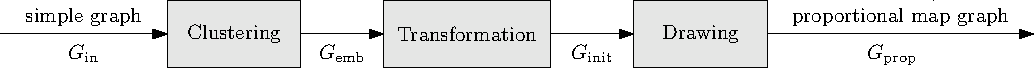
\includegraphics[width=0.9\textwidth]{Resources/Pipeline-Application-Static.pdf}
	\caption{Overview of a possible algorithmic pipeline for generic applications.}
	\label{fig:static-pipeline-application}
\end{figure}

We will now discuss our implementation of the transformation and drawing phases of the pipeline in detail.

\clearpage
\section{Transformation to Polygonal Dual}
\label{sect:transformation-to-dual}

In this step of the pipeline, we take a filtered cluster graph \clustergraph{} and form a polygonal dual of thereof, resulting in the map \initmap{}.
To formalize the their relationship, we need the concept of the augmented dual:

\begin{definition}
The \emph{augmented dual} $G^+$ of a plane graph $G$ is the plane multigraph obtained by first placing a new vertex $v^+$ in the outer face of $G$, connecting it to all vertices on the outer face, in order, without introducing edge crossings, and then forming its dual.
\label{def:augmented-dual}
\end{definition}

\Cref{fig:transformation-augmented-dual} illustrates how the augmented dual $G^+$ of a plane graph $G$ (\cref{subfig:transformation-augmented-dual-1}) is formed.
We add the helper vertex $v^+$ and helper edges $\{v^+,\cdot\}$ in the outer face in \cref{subfig:transformation-augmented-dual-2}.
We draw the helper edges as in \cite{wagner2016algorithmen} because it does not matter where in the plane this helper vertex lies \emdash{} all that matters is that each pair of adjacent vertices on the outer face forms a new triangular face with $v^+$.
In \cref{subfig:transformation-augmented-dual-3}, we overlay the dual vertices and edges in red.
\Cref{subfig:transformation-augmented-dual-4} shows just the augmented dual of $G$.
%
\begin{figure}[H]
	\centering
	\subfigure[]{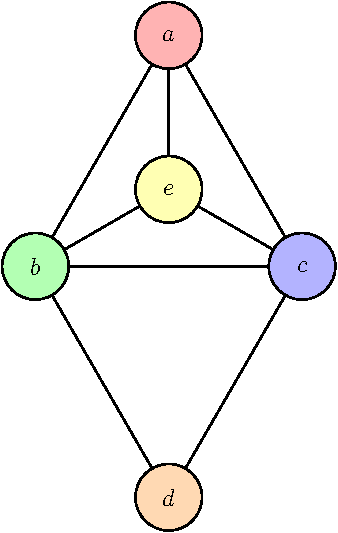
\includegraphics[height=130px]{Resources/Transformation-AugmentedDual-1.pdf}\label{subfig:transformation-augmented-dual-1}}
	\quad
	\subfigure[]{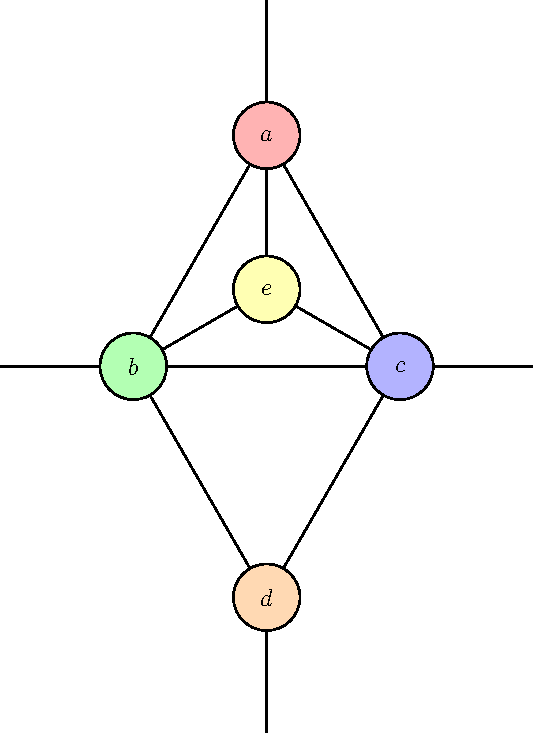
\includegraphics[height=130px]{Resources/Transformation-AugmentedDual-2.pdf}\label{subfig:transformation-augmented-dual-2}}
	\quad
	\subfigure[]{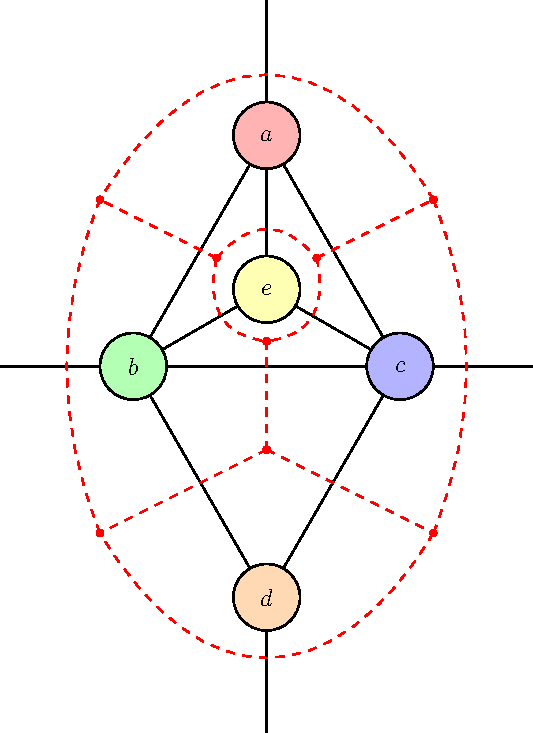
\includegraphics[height=130px]{Resources/Transformation-AugmentedDual-3.pdf}\label{subfig:transformation-augmented-dual-3}}
	\quad
	\subfigure[]{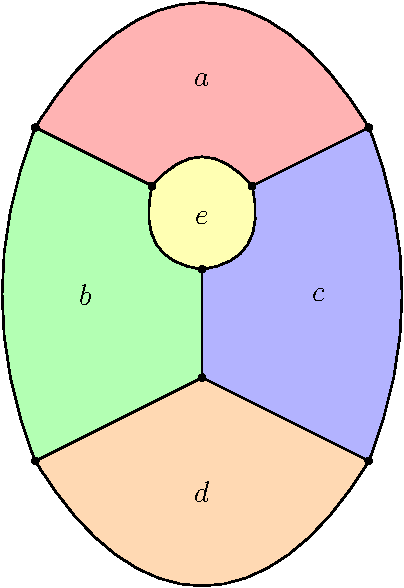
\includegraphics[height=130px]{Resources/Transformation-AugmentedDual-4.pdf}\label{subfig:transformation-augmented-dual-4}}
	\caption{Step-by-step representation of forming a plane graph's augmented dual.}
	\label{fig:transformation-augmented-dual}
\end{figure}

Note that analogous to the regular dual, the weak dual of the augmented dual of a plane graph $G$ is $G$ again, \ie{} $(G^+)^- = G$.

The augmented dual $G^+$ (\cref{subfig:transformation-augmented-dual-4}) of a biconnected and internally triangulated plane graph $G$ (\cref{subfig:transformation-augmented-dual-1}) essentially is a contact representation thereof.
In a polygonal dual, however, the edges cannot be curves and must be polylines instead.
The map \initmap{} can therefore be interpreted as a subdivision of the augmented dual $(\clustergraph{})^+$ in combination with a planar straight-line drawing thereof.



\paragraph{Algorithm Overview}

The underlying idea of creating the initial map \initmap{} is as follows:
Given a filtered cluster graph \clustergraph{}, we place vertices on edges of the outer face of \clustergraph{} (those edges bound additional triangular faces after adding the helper vertex in the process of forming the augmented dual) and inside the internal faces of \clustergraph{}.
We then connect these vertices if their corresponding faces are adjacent.
Connecting two vertices may require additional subdivision vertices or bends in order not to introduce edge crossings \emdash{} we use a single bend per edge.

The following figure illustrates an example:
%
\begin{figure}[H]
	\centering
	\subfigure[]{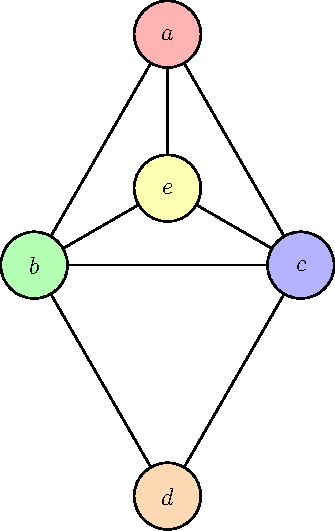
\includegraphics[height=70mm]{Resources/Transformation-Algorithm-1.pdf}\label{subfig:transformation-algorithm-1}}
	\quad
	\subfigure[]{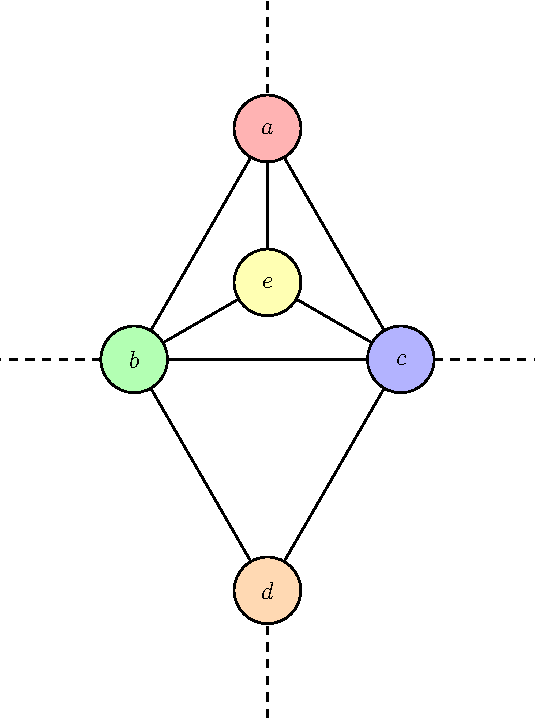
\includegraphics[height=70mm]{Resources/Transformation-Algorithm-2.pdf}\label{subfig:transformation-algorithm-2}}
	\quad
	\subfigure[]{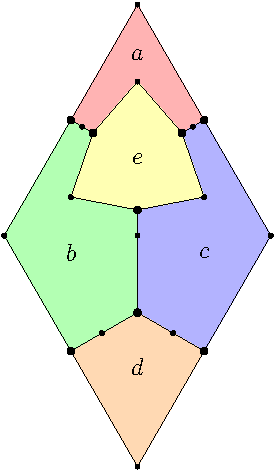
\includegraphics[height=70mm]{Resources/Transformation-Algorithm-3.pdf}\label{subfig:transformation-algorithm-3}}
	\caption{A filtered cluster graph \clustergraph{} (a), the helper graph \clustergraph{+} (b), and the polygonal dual \initmap{} of \clustergraph{} as produced by \cref{alg:transformation-to-dual} (c).}
	\label{fig:transformation-algorithm}
\end{figure}

Before feeding the filtered cluster graph \clustergraph{} into the algorithm, we construct a planar straight-line drawing \clusterdrawing{} of \clustergraph{} with the same planar embedding.
According to Fáry's theorem \cite{fary1948straight} \cite{wagner1936bemerkungen} \cite{stein1951convex}, such a drawing exists for every plane graph.
There are numerous popular algorithms to construct such a drawing, \eg{} Tutte's method \cite{tutte1963draw}, the shift method \cite{fraysseix1990draw}, or the Schnyder realizer method \cite{schnyder1990embedding}.



\clearpage
\paragraph{Algorithm Implementation}

\begin{algorithm}[H]
  \caption{Transformation to Polygonal Dual}
  \label{alg:transformation-to-dual}
  \SetKwData{Endpoints}{endpoints}
  \SetKwFunction{Appending}{appending}
  \SetArgSty{textrm}
  \vspace{5pt}
  \KwData{filtered cluster graph \clustergraph{} and a planar straight-line drawing \clusterdrawing{} thereof}
  \KwResult{polygonal dual \initmap{} of \clustergraph{}, in the form of a 1-subdivision of the augmented dual of \clustergraph{} and planar straight-line drawing thereof}
  \BlankLine
  create empty contact representation \initmap{}\;
  \BlankLine
  \tcp{compute dual vertices and edges}
  \ForEach{internal face $f$ in \clustergraph{}}{
    \label{line:transformation-loop1-start}
    add \quoted{internal face vertex} $v_f$ to \initmap{}\; \label{line:transformation-innerfacevertex}
    position $v_f$ at barycenter of $f$ in \clustergraph{} \label{line:transformation-barycenter1}\;
    \label{line:transformation-loop1-end}
  }
  \ForEach{edge $\{u,v\}$ in \clustergraph{}}{
    \label{line:transformation-loop2-start}
  	\If{$\{u,v\}$ is incident to two different internal faces $f, g$ in \clustergraph{} \label{line:transformation-incidentfacelookup1}}{
  	  add \quoted{subdivision vertex} $v_\text{sub}$ to \initmap{}\; \label{line:transformation-subdivisionvertex1}
  	  position $v_\text{sub}$ at midpoint of ${\{u,v\}}$ in \clustergraph{}\;
  	  add edge between $v_f$ and $v_\text{sub}$ to \initmap{}\; \label{line:transformation-edgetype1-start}
  	  add edge between $v_\text{sub}$ and $v_g$ to \initmap{}\; \label{line:transformation-edgetype1-end}
  	}
  	\ElseIf{$\{u,v\}$ is incident to a single internal face $f$ in \clustergraph{} \label{line:transformation-incidentfacelookup2}}{
  	  add \quoted{outer edge vertex} $v_{\{u,v\}}$ to $G_\text{init}$\; \label{line:transformation-outeredgevertex}
  	  position $v_{\{u,v\}}$ at midpoint of ${\{u,v\}}$ in \clustergraph{}\;
  	  add \quoted{subdivision vertex} $v_\text{sub}$ to \initmap{}\; \label{line:transformation-subdivisionvertex2}
  	  position $v_\text{sub}$ at midpoint of segment between barycenter of $f$ and midpoint of ${\{u,v\}}$ in \clustergraph{} \label{line:transformation-barycenter2}\;
  	  add edge between $v_{\{u,v\}}$ and $v_\text{sub}$ to \initmap{}\; \label{line:transformation-edgetype2-start}
  	  add edge between $v_\text{sub}$ and $v_f$ to \initmap{}\; \label{line:transformation-edgetype2-end}
  	}
  	\label{line:transformation-loop2-end}
  }
  \ForEach{incident edges $\{\{u,v\},\{v,w\}\}$ on outer face of \clustergraph{}}{
    \label{line:transformation-loop3-start}
    add \quoted{subdivision vertex} $v_\text{sub}$ to \initmap{}\; \label{line:transformation-subdivisionvertex3}
    position $v_\text{sub}$ at position of $v$ in \clustergraph{}\;
    add edge between $v_{\{u,v\}}$ and $v_\text{sub}$ to \initmap{}\; \label{line:transformation-edgetype3-start}
    add edge between $v_\text{sub}$ and $v_{\{v,w\}}$ to \initmap{}\; \label{line:transformation-edgetype3-end}
    \label{line:transformation-loop3-end}
  }
  \BlankLine
  \tcp{compute faces in \initmap{} and match them to vertices in \clustergraph{}}
  \ForEach{vertex $u$ in \clustergraph{} \label{line:transformation-enumeratevertices}}{
    \label{line:transformation-loop4-start}
    $\Endpoints \gets ()$\;
    \ForEach{adjacent pair $(v,w)$ of neighbors of $u$ in counterclockwise order \label{line:transformation-enumerateedges}}{
      \If{$(u,v,w)$ bound a triangular face $f$ in counterclockwise order in \clustergraph{} \label{line:transformation-checktriangle}}{
        append $v_f$ to \Endpoints\;
      }
      \Else{
        append $v_{\{u,v\}}$ to \Endpoints\;
        append $v_{\{u,w\}}$ to \Endpoints\;
      }
    }
    \ForEach{adjacent pair $(v,w)$ in \Endpoints \label{line:transformation-insertsubdivisions}}{
      insert subdivision vertex connecting $v$ to $w$ between $v$ and $w$ in \Endpoints\;
    }
    define $f_u$ as internal face on \Endpoints in \initmap{}\;
    set weight of $f_u$ in \initmap{} to weight of $u$ in \clustergraph{}\;
    \label{line:transformation-loop4-end}
  }
  \Return \initmap{}
\end{algorithm}
\vfill



\paragraph{Algorithm Correctness}

We show the algorithm's correctness in two steps.
First, we show that the algorithm does indeed construct a 1-subdivision of the augmented dual of \clustergraph{}.
Second, we show that the constructed drawing thereof is planar, making it a contact representation of \clustergraph{} as previously explained and illustrated in \cref{fig:transformation-augmented-dual}.

Recall that $(\clustergraph{})^+$ is a contact representation of \clustergraph{}.
We can construct $(\clustergraph{})^+$ via a helper graph \clustergraph{+} that we obtain by inserting a helper vertex $v^+$ in the outer face of \clustergraph{} and connecting it to all vertices on the outer face of \clustergraph{}, in order, without introducing edge crossings.
The contact representation $(\clustergraph{})^+$ then is the regular dual of \clustergraph{+}, \ie{} $(\clustergraph{})^+ = (\clustergraph{+})^*$.
By adding the helper vertex $v^+$ and helper edges $\{v^+,\cdot\}$, the edges on the outer face of \clustergraph{} bound new triangular faces of \clustergraph{+}.

The dual of a plane graph has vertices in each of the primal graph's faces.
We place these vertices in the original internal faces in \cref{line:transformation-innerfacevertex} and in \emdash{} or rather on \emdash{} the new triangular faces in \clustergraph{+} in \cref{line:transformation-outeredgevertex}.
Vertices in the dual are adjacent if their respective faces are adjacent in the primal.
Thus for every edge separating two faces in the primal \clustergraph{+}, we require a dual edge in $(\clustergraph{+})^*$.
We add these edges in \crefrange{line:transformation-edgetype1-start}{line:transformation-edgetype1-end} (for adjacent internal faces in \clustergraph{}), in \crefrange{line:transformation-edgetype2-start}{line:transformation-edgetype2-end} (for edges separating an internal face in \clustergraph{} from a new face in \clustergraph{+}), and in \crefrange{line:transformation-edgetype3-start}{line:transformation-edgetype3-end} (for helper edges $\{v^+,\cdot\}$ separating two new faces in \clustergraph{+}).
Because we place all bends of the dual edges on the respective primal edge, the cyclic order of the edges incident to each vertex is equivalent to the cyclic order of the edges bounding the respective faces in the primal.

\begin{figure}[H]
	\centering
	\subfigure[]{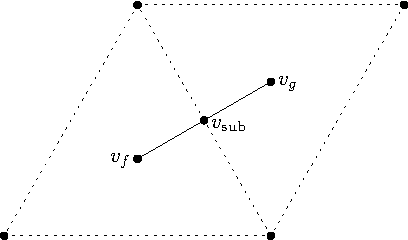
\includegraphics[height=32mm]{Resources/Transformation-DualEdgeConstruction-1.pdf}\label{subfig:transformation-dual-edge-construction-1}}
	\subfigure[]{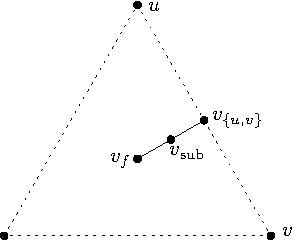
\includegraphics[height=32mm]{Resources/Transformation-DualEdgeConstruction-2.pdf}\label{subfig:transformation-dual-edge-construction-2}}
	\quad
	\subfigure[]{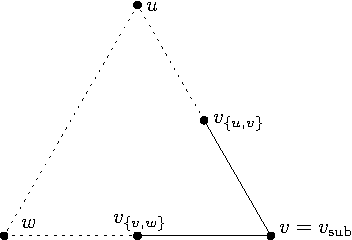
\includegraphics[height=32mm]{Resources/Transformation-DualEdgeConstruction-3.pdf}\label{subfig:transformation-dual-edge-construction-3}}
	\caption{Construction of the dual edges as per \cref{alg:transformation-to-dual} between two internal faces in \clustergraph{} (a), between an internal face of \clustergraph{} and a new face in \clustergraph{+} (b), and between two new faces in \clustergraph{+} (c). The dotted lines are edges in \clustergraph{}.}
	\label{fig:transformation-dual-edge-construction}
\end{figure}

It is left to show that the placement of vertices and edges produces a crossing-free drawing.
To do so, we consider the edges from non-subdivision vertices in $(\clustergraph{+})^*$ to their neighbors.
Recall that those vertices correspond to faces in \clustergraph{+}.
Following the construction illustrated in \crefrange{subfig:transformation-dual-edge-construction-1}{subfig:transformation-dual-edge-construction-2}, the three incident edges to a vertex corresponding to an internal face of \clustergraph{} lie completely inside said face.
Because these edges go straight towards the midpoint of the incident edges, they don't self-intersect.

The vertices corresponding to new faces in \clustergraph{+} lie on the midpoint of the bounding edge that already exists in \clustergraph{}.
The dual edges connecting two of those vertices are constructed such that they partition the boundary of the outer face of \clustergraph{} (see \cref{subfig:transformation-dual-edge-construction-3}) and therefore don't intersect any of the edges discussed so far.
Their edge to the vertex corresponding to the adjacent internal face goes straight towards said vertex, meeting it halfway, as illustrated in \cref{subfig:transformation-dual-edge-construction-2}.
Because some $v_f$'s incident edges all go straight towards its bounding edges as outlined above, this kind of edge does not introduce any edge crossings either.
The constructed graph and drawing is therefore a 1-subdivision of the augmented dual of \clustergraph{} and the drawing is planar.

Once the algorithm has constructed \initmap{}, we compute an explicit representation of its internal faces and the corresponding vertices in the primal.
We do so for the augmented dual $(\clustergraph{})^+$ first (loop in \cref{line:transformation-enumerateedges}) and then insert the subdivision vertices (loop in \cref{line:transformation-insertsubdivisions}).
The face in $(\clustergraph{})^+$ that corresponds to a vertex $v$ of \clustergraph{} is bounded by vertices corresponding to internal faces of \clustergraph{} that contain $v$, plus the vertices corresponding to the additional triangular faces in \clustergraph{+} in case $v$ lies on outer face of \clustergraph{}.
Iterating over adjacent pairs $(e_1, e_2)$ of incident edges in counterclockwise order correctly detects the internal faces between $e_1$ and $e_2$ and the case where $e_1$ and $e_2$ wrap around on the outside, in order.
The orientation check in \cref{line:transformation-checktriangle} is required such that the wraparound case isn't misclassified as an internal face.
This would be the case for internal faces of \clustergraph{} with two edges on the outer face, as is the case for vertex $v \coloneqq d$ and edges $e_1 \coloneqq \{d,b\}, e_2 \coloneqq \{d,c\}$ in \cref{fig:transformation-algorithm}.



\paragraph{Algorithm Runtime}

To compute the input graph's faces, we replace every edge with two inversely oriented, directed edges.
We then repeatedly pick any unmarked edge and form a directed cycle by following the next outgoing edge according to the embedding, marking the edges as we go.
Once all edges have been marked, we have found all faces.
The outer face is the one face whose interior is on the left when traveling along its bounding edges.
This can be implemented in $\bigTheta{n+m}$, where $n = \lvert V(\clustergraph{}) \rvert$ and $m = \lvert E(\clustergraph{}) \rvert$.

The input graph has $\bigTheta{n}$ internal faces and they are all triangles, therefore we can compute their barycenter in $\bigTheta{1}$ each (\cref{line:transformation-barycenter1}, \cref{line:transformation-barycenter2}).
By keeping track of of which faces an edge of the input graph is incident to while computing the faces as outlined above, we allow for $\bigTheta{1}$ lookups in \cref{line:transformation-incidentfacelookup1} and \cref{line:transformation-incidentfacelookup2}.
The loop in \crefrange{line:transformation-loop1-start}{line:transformation-loop1-end} therefore runs in $\bigTheta{n}$, the loop in \crefrange{line:transformation-loop2-start}{line:transformation-loop2-end} in $\bigTheta{m}$, and the loop in \crefrange{line:transformation-loop3-start}{line:transformation-loop3-end} in $\bigTheta{m}$.

The loop in \crefrange{line:transformation-loop4-start}{line:transformation-loop4-end} processes every vertex once in \cref{line:transformation-enumeratevertices} and and every edge twice \cref{line:transformation-enumerateedges}.
We can check if the vertices $u,v,w$ form a triangle in constant time (\cref{line:transformation-checktriangle}) by checking if there's an edge between $v$ and $w$.
Considering each of the $\bigTheta{n+m}$ vertices of the generated graph appears in \code{endpoints} in no more than two iterations of the loop in \crefrange{line:transformation-loop4-start}{line:transformation-loop4-end} and all those vertices have degree 3, we can find their shared neighbor in constant time and implement the entire loop to run in $\bigTheta{n+m}$.

The entire algorithm can therefore be implemented to run in $\bigTheta{n+m}$.



\paragraph{Theoretical Bounds}

But do we have to subdivide edges of the augmented dual of our filtered cluster graph \clustergraph{} in order to get a valid polygonal dual of \clustergraph{}?
Although the augmented dual $(\clustergraph{})^+$ is plane by definition, it is not immediately obvious that there exists a planar straight-line drawing of $(\clustergraph{})^+$ \emdash{} and that's what we need for it to be a polygonal contact representation.

In our case, however, $(\clustergraph{})^+$ is simple, \ie{} there are no loops or multiple adjacencies.
Recall that \clustergraph{} is biconnected and internally triangulated.
Adding the helper vertex in the outer face of \clustergraph{} and connecting it to all vertices on the outer face therefore creates a fully triangulated, simple graph.
In a simple triangulated graph, there are no two edges that are incident to the same faces (only those would create multiple adjacencies when forming the dual) and no edges that have the same face on both sides (only those would create loops when forming the dual) either.
The augmented dual $(\clustergraph{})^+$ is therefore simple and, according to Fáry's theorem \cite{fary1948straight}, there exists a planar straight-line drawing of $(\clustergraph{})^+$ respecting its original planar embedding.

In addition to having a planar straight-line drawing, $(\clustergraph{})^+$ is also a cubic graph, \ie{} one in which all vertices have degree 3.
This is because \clustergraph{} with the helper vertex is a triangulated graph, meaning every face is incident to exactly three edges, which turns into every vertex being incident to exactly three edges when forming the dual.
According to the results of Thomassen \cite{thomassen1992plane}, $(\clustergraph{})^+$ is therefore area-universal.
This means that regardless of the concrete face weights that \clustergraph{} prescribes, there exists a planar straight-line drawing of $(\clustergraph{})^+$ realizing those weights/areas.

Even without subdividing edges in $(\clustergraph{})^+$, we could therefore choose the map \initmap{} in such a way that it has perfect statistical accuracy already.
Such a drawing of $(\clustergraph{})^+$ is non-trivial to compute though and creates undesired region shapes according to our other quality metrics.
Instead, the algorithm we proposed here subdivides all edges of the augmented dual $(\clustergraph{})^+$ once and leaves us with a decent initial drawing and enough degrees of freedom to optimize for other quality metrics in \cref{sect:drawing-the-dual}.


\clearpage
\section{Drawing the Polygonal Dual}
\label{sect:drawing-the-dual}

In the second step of the pipeline, we apply a force-directed graph drawing algorithm to the initial map graph $G_\text{init}$ produced by \cref{alg:transformation-to-dual} to generate the approximately area-proportional map graph $G_\text{prop}$.

In a force-directed algorithm, we interpret a graph's vertices as particles in a physical system.
Based on the structure of the graph and the relative position of the particles, we define several forces that act to bring the system to a stable equilibrium position in which its potential energy is at a local minimum.
In these equilibrium positions, the system is in a somewhat relaxed state that, in the context of graph drawing, generally is a visually appealing drawing of the graph.
We find an equilibrium position by iteratively computing the net force acting on each particle and displacing it by a small amount in the direction of the net force, based on its absolute value.



\paragraph{Forces}

%https://slideplayer.com/slide/4924642/
%v-v-rep: Eades 1984, Fruchterman & Reingold
%v-e-rep: Davidson & Harel 1996, Bertault 1999

We define the forces that exist in our particle system with two goals in mind:
First, the faces of the graph (the regions of the map) to have an area ought to be close to proportional to some prescribed value.
Second, we want the faces to be \emph{locally fat}.
Our intuitive understanding of local fatness is that a region shouldn't have drawn-out, tight corridors.
We formalize and discuss different quantifiable measures that aim to capture the local fatness of regions in \cref{chap:evaluation}.
Note that both of these are soft requirements.
Planarity of the resulting drawing, on the other hand, is a hard requirement that must be preserved at all costs.

Let us now discuss the concrete force components that act to bring our particle system to an equilibrium position.
%
\begin{itemize}
\item \textbf{Air Pressure:} % alam2013computing
Motivated by Alam \etal{} \cite{alam2013computing}, we treat the polygonal regions as volumes of some amount of air equal to the respective face's weight.
This allows us to define an analog to air pressure in the polygonal regions that exerts forces on the regions' edges.
This force is responsible for growing faces that are currently compressed and shrinking faces that are currently larger than they should be, therefore working towards the statistical accuracy of the generated map.

We want this force and the overall drawing to be agnostic to constant factors of the face weights and therefore compute the normalized pressure $P(f)$ in an internal face $f$ as
%
\begin{equation*}
	P(f) \coloneqq \frac{w(f)}{A(f)} \cdot \frac{\sum_{g \in F}{A(g)}}{\sum_{g \in F}{w(g)}},
\end{equation*}
%
where $A(f)$ is the area currently covered by some internal face $f$ and $w(f)$ its weight.
We set the normalized pressure in the outer face to the weighted average normalized pressure, \ie{}
%
\begin{equation*}
	P(f_\text{outer}) \coloneqq \frac{\sum_{f \in F}{A(f) \cdot P(f)}}{\sum_{f \in F}{A(f)}} = 1.
\end{equation*}

Physical pressure is the ratio of force to area.
The air pressure in each of the regions $f$ therefore exerts a force on each bounding edge $e = \{u,v\}$ based on the pressure's magnitude and the edge's length $l(e)$ in relation to the entire region's boundary's length $l(f)$.
We orient $e = \{u,v\}$ such that $u$ directly precedes $v$ on the boundary of $f$ and define the force as
%
\begin{equation}
	\vec{F}_P((u,v);f) \coloneqq
	3 \cdot P(f)\cdot\frac{l(e)}{l(f)}
	\cdot \Norm(\Perp(\longvec{vu}))
	,
\end{equation}
%
where $\Perp(\cdot)$ rotates a vector by $90^\circ$ in counterclockwise direction and $\Norm(\cdot)$ normalizes a vector to unit length.
We apply $\vec{F}_P(\{u,v\};f)$ to both endpoints $u$ and $v$ of the edge, as illustrated in \cref{fig:drawing-forces-air-pressure}.

\begin{figure}[H]
	\centering
	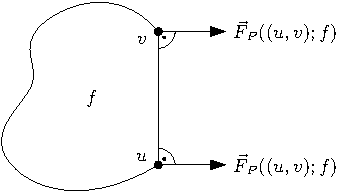
\includegraphics[height=35mm]{Resources/Drawing-Forces-AirPressure.pdf}
	\caption{Forces exerted on the endpoints of the edge $e = \{u,v\}$ by the air pressure in the region $f$.}
	\label{fig:drawing-forces-air-pressure}
\end{figure}

Considering every edge is incident to exactly two faces, we can write the net force exerted on an oriented edge $e = (u,v)$ incident to face $f$ on the left and face $g$ on the right as
%
\begin{equation*}
	\vec{F}_P((u,v);f,g) \coloneqq
	3 \cdot \left( P(g)\cdot\frac{l(e)}{l(g)} - P(f)\cdot\frac{l(e)}{l(f)} \right)
	\cdot \Norm(\Perp(\longvec{uv}))
	,
\end{equation*}
%
matching the force that Alam \etal{} \cite{alam2013computing} use for computing their cartograms.


\item \textbf{Angular Resolution:} % argyriou2013maximizing
Internal face angles close to $0^\circ$ cause tight corridors in the form of pointy spikes and angles close to $360^\circ$ the opposite \emdash{} both features we want to avoid if possible.
We therefore define a force that optimizes angular resolution, \ie{} a force that tries to evenly distribute the angles formed by the incident edges around a vertex $v$ at $\frac{360^\circ}{\deg(v)}$ each.

Let $v$ be a vertex and let $u$ and $w$ be two successive neighbors of $u$ in counterclockwise order.
Also let $\measuredangle_{uvw} \in \lbrack 0^\circ, 360^\circ )$ denote the normalized angle from $u$ via $v$ to $w$ measured in counterclockwise direction.
%Analogous to \cite{argyriou2013maximizing}, we define an angular force
With this, we define the force $\vec{F}_\measuredangle(v;u,w)$ as
%
\begin{equation}
	\vec{F}_\measuredangle(v;u,w) \coloneqq
	\frac{1}{2} \cdot \frac{\frac{360^\circ}{\deg(u)} - \measuredangle_{uvw}}{\measuredangle_{uvw}}
	\cdot \Bsc(\angle_{uvw})
	.
\end{equation}

Here $\Bsc(\angle_{uvw})$ computes the normalized bisector of the given angle, \ie{} $\Norm(\longvec{vu})$ rotated by $\frac{1}{2} \measuredangle_{uvw}$ in counterclockwise direction.
The construction of $\vec{F}_\measuredangle(v;u,w)$ is illustrated in \cref{fig:drawing-forces-angular-resolution}.

\begin{figure}[H]
	\centering
	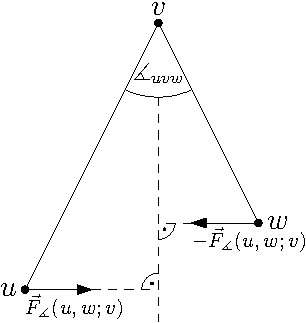
\includegraphics[height=40mm]{Resources/Drawing-Forces-AngularResolution.pdf}
	\caption{Force exerted on some vertex $v$ with successive neighbors $u$ and $w$ of $v$ where $\measuredangle_{uvw} > \frac{360^\circ}{\deg(v)}$.}
	\label{fig:drawing-forces-angular-resolution}
\end{figure}

For all triplets $(u,v,w)$ of vertices $v$ and successive neighbors $u$, $w$ of $v$, we apply $\vec{F}_\measuredangle(v;u,w)$ to $v$.
If the angle at $v$ is currently too small, the force acts to move $v$ along the bisector, thereby increasing the angle; otherwise it acts to move $v$ against the bisector, thereby decreasing the angle.

Argyriou \etal{} \cite{argyriou2013maximizing} use a similar force to obtain uniform angles around all vertices.
However, instead of applying the force to the vertex $v$ whose angular resolution we want to improve as we do, they apply perpendicular forces to its neighbors.
In our tests, the approach of Argyriou \etal{} has shown not to converge well due to us not having a force acting towards a uniform edge length, as discussed below in a bit.


\item \textbf{Vertex-vertex repulsion:} % eades84heuristic
We define a repulsive force between pairs of vertices to prevent the vertices from clumping together.
This is important because in order to preserve planarity, vertices that are very close to others will need to have their movement restricted severely, possibly hindering us from satisfying our aesthetic criteria.
We think of the vertices as charged particles that push each other away and define a repulsive force based on Coulomb's law that is exerted along the line connecting pairs of vertices and whose magnitude depends on their Euclidean distance:
%
\begin{equation}
	\vec{F}_\leftrightarrow(u;v) \coloneqq
	25 \cdot \frac{1}{\norm{\longvec{uv}}^2}
	\cdot \Norm(\longvec{uv})
\end{equation}

For pairs $(u, v) \in V^2, u \neq v$, we apply $\vec{F}_\leftrightarrow(u;v)$ to $u$.
We restrict ourselves to pairs $(u,v)$ where $u$ and $v$ lie together on the boundary of some face for performance reasons and because for other pairs, there'd be other vertices or edges between $u$ and $v$ that would push the two vertices apart.

This kind of force was first used by Eades \cite{eades84heuristic}, albeit only for non-adjacent pairs of vertices.
We apply this force to adjacent vertices as well because we don't use spring-like forces between adjacent vertices trying to achieve a uniform edge length (and therefore some non-zero distance) as Eades does, as discussed below.


\item \textbf{Vertex-edge repulsion:} % bertault1999force
In another attempt to prevent tight corridors from forming, we define an additional repulsive force between vertices and edges.
Given an edge $e = \{u,w\}$ and non-incident vertex $v$, we define $v_+$ as the point on the segment from $u$ to $w$ with the smallest Euclidean distance to $v$.
We then define the repulsive force as
%
\begin{equation}
	\vec{F}_\bot(v;\{u,w\}) \coloneqq
	10 \cdot \frac{1}{\norm{\longvec{v_+v}}^2}
	\cdot \abs{\vec{n}_e \cdot \Norm(\longvec{v_+v})}
	\cdot \Norm(\longvec{v_+v})
	,
\end{equation}
%
where $\vec{n}_e$ is the normalized normal vector of the edge $e$ pointing in either direction.
The following figure illustrates the construction of the force $\vec{F}_\bot(v;\{u,w\})$:
%
\begin{figure}[H]
	\centering
	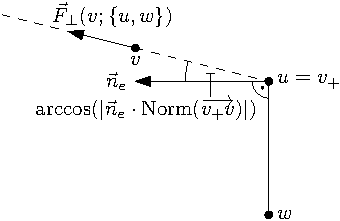
\includegraphics[height=40mm]{Resources/Drawing-Forces-VertexEdgeRepulsion.pdf}
	\caption{Force exerted on some vertex $v$ by a non-incident edge $\{u,w\}$.}
	\label{fig:drawing-forces-vertex-edge-repulsion}
\end{figure}

Analogous to the vertex-vertex-repulsion discussed above, we compute the force $\vec{F}_\bot(v;\{u,w\})$ only for vertices and edges that lie together on the boundary of some face and apply it to $v$.

This repulsive force is very similar to what Bertault uses in PrEd \cite{bertault1999force}.
However, we have an additional dot product term for how $v$ is positioned relatively to the edge $\{u,w\}$ whereas Bertault drops the force altogether if the orthogonal projection of $v$ onto the line through $u$ and $w$ doesn't lie between $u$ and $w$.
In our tests, Bertault's definition resulted in very unstable simulations as these force swayed back and forth between having full impact and no impact at all.
\end{itemize}

The constant factors of the force components above were determined experimentally and yielded good results for a variety of randomly generated graphs.

Note that we do not define attractive forces between adjacent vertices as most traditional force-directed algorithms do.
Such an attractive force is generally used to keep adjacent vertices close together while nonadjacent vertices are pushed further apart by the repulsive forces.
This works for many graph drawing algorithms because for them, uniform edge length is a desired feature in equilibrium.
In our case, however, there is no correlation between the extent of a region and the number of edges on its boundary and, subsequently, the length of the edges on its boundary.
Including such an attractive force here would in fact be counterproductive.

To make sure that the physical simulation converges, we cool the particle system down over time.
We define a global cooling parameter $\alpha = 0.01$ and, at step $i$ of the iterative process, add $(1 - \alpha)^i$ as a factor to all of the forces mentioned above.
By doing so, we prevent unstable oscillations around equilibrium.

In our implementation, we also smooth vertices of degree 2 that become too close to other vertices and subdivide edges that become too long in order to create more degrees of freedom in the respective face's shape.
To do so, we first compute the average edge length $\bar{l}$ as
%
\begin{equation*}
	\bar{l} \coloneqq \frac1{\abs{E}} \cdot \sum\limits_{e \in E} l(e)
	.
\end{equation*}
%
Then, at each iteration, we subdivide edges that are longer than $2\bar{l}$ at their midpoint and smooth vertices whose distance to the closest other vertex is $\frac{1}{10}\bar{l}$ or less if we can do so without introducing edge crossings.



\paragraph{Preventing Edge Crossings}

When iteratively displacing the map graph's vertices according to the forces defined above, we must pay close attention to not accidentally introduce edge crossings.

To do so, we adopt the rules of ImPrEd \cite{simonetto2011impred} that ensure no edge crossings are created.
At each step of the algorithm, ImPrEd computes the maximum distance each of the vertices is allowed to move such that the drawing's edge crossing properties are guaranteed to be preserved.
The maximum displacement per vertex is computed in eight general directions, zones of $45^\circ$ each.
The actual displacement of the vertices is then clamped at the maximum distance the vertex can safely move in the desired direction.

